\documentclass[tikz,border=8pt]{standalone}
% Shared look for every TikZ diagram. Load with % Shared look for every TikZ diagram. Load with % Shared look for every TikZ diagram. Load with \input{../../tools/tikz-style.tex}
\usepackage[T1]{fontenc}
\usepackage{lmodern}
\renewcommand{\sfdefault}{lmr}  % diagrams use the same serif as the text
\usetikzlibrary{arrows.meta, positioning, shapes.geometric, calc, fit, backgrounds}
\definecolor{cblue}{HTML}{4C78A8}
\definecolor{corange}{HTML}{F58518}
\definecolor{cgreen}{HTML}{54A24B}
\definecolor{cred}{HTML}{E45756}
\definecolor{cpurple}{HTML}{B279A2}
\definecolor{cgrey}{HTML}{6B6B6B}
\tikzset{
  every picture/.style={font=\sffamily, line width=1.2pt},
  box/.style={draw=#1, fill=#1!12, rounded corners=4pt, align=center, inner sep=7pt, minimum height=1.1cm},
  box/.default=cgrey,
  arrow/.style={-{Stealth[length=3mm]}, draw=cgrey, line width=1.4pt},
  title/.style={font=\sffamily\bfseries\Large},
  note/.style={font=\sffamily\small, text=cgrey, align=center},
}
\AtBeginDocument{\hyphenpenalty=10000 \exhyphenpenalty=10000}

\usepackage[T1]{fontenc}
\usepackage{lmodern}
\renewcommand{\sfdefault}{lmr}  % diagrams use the same serif as the text
\usetikzlibrary{arrows.meta, positioning, shapes.geometric, calc, fit, backgrounds}
\definecolor{cblue}{HTML}{4C78A8}
\definecolor{corange}{HTML}{F58518}
\definecolor{cgreen}{HTML}{54A24B}
\definecolor{cred}{HTML}{E45756}
\definecolor{cpurple}{HTML}{B279A2}
\definecolor{cgrey}{HTML}{6B6B6B}
\tikzset{
  every picture/.style={font=\sffamily, line width=1.2pt},
  box/.style={draw=#1, fill=#1!12, rounded corners=4pt, align=center, inner sep=7pt, minimum height=1.1cm},
  box/.default=cgrey,
  arrow/.style={-{Stealth[length=3mm]}, draw=cgrey, line width=1.4pt},
  title/.style={font=\sffamily\bfseries\Large},
  note/.style={font=\sffamily\small, text=cgrey, align=center},
}
\AtBeginDocument{\hyphenpenalty=10000 \exhyphenpenalty=10000}

\usepackage[T1]{fontenc}
\usepackage{lmodern}
\renewcommand{\sfdefault}{lmr}  % diagrams use the same serif as the text
\usetikzlibrary{arrows.meta, positioning, shapes.geometric, calc, fit, backgrounds}
\definecolor{cblue}{HTML}{4C78A8}
\definecolor{corange}{HTML}{F58518}
\definecolor{cgreen}{HTML}{54A24B}
\definecolor{cred}{HTML}{E45756}
\definecolor{cpurple}{HTML}{B279A2}
\definecolor{cgrey}{HTML}{6B6B6B}
\tikzset{
  every picture/.style={font=\sffamily, line width=1.2pt},
  box/.style={draw=#1, fill=#1!12, rounded corners=4pt, align=center, inner sep=7pt, minimum height=1.1cm},
  box/.default=cgrey,
  arrow/.style={-{Stealth[length=3mm]}, draw=cgrey, line width=1.4pt},
  title/.style={font=\sffamily\bfseries\Large},
  note/.style={font=\sffamily\small, text=cgrey, align=center},
}
\AtBeginDocument{\hyphenpenalty=10000 \exhyphenpenalty=10000}

\begin{document}
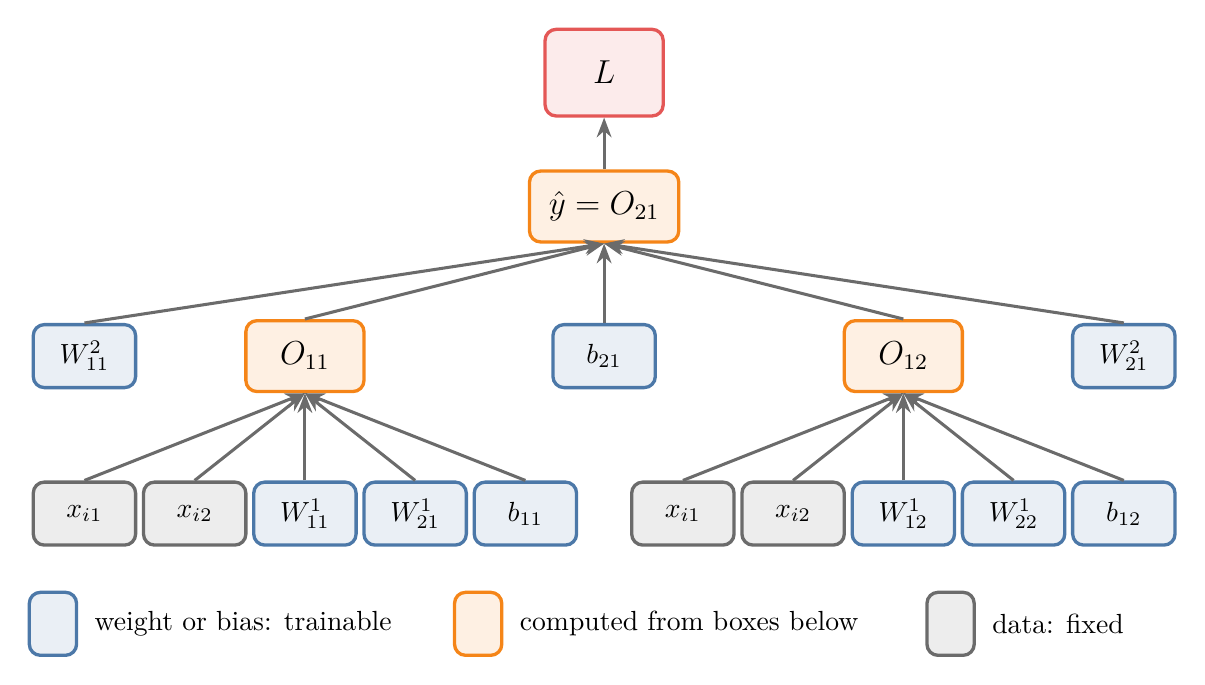
\begin{tikzpicture}[
  comp/.style={box=corange, minimum width=1.5cm, minimum height=0.9cm, font=\sffamily\large},
  par/.style={box=cblue, minimum width=1.3cm, minimum height=0.8cm, inner sep=4pt},
  dat/.style={box=cgrey, minimum width=1.3cm, minimum height=0.8cm, inner sep=4pt},
  dep/.style={-{Stealth[length=2.5mm]}, draw=cgrey, line width=1.1pt}]
  \node[box=cred, minimum width=1.5cm, font=\sffamily\large] (L) at (0, 0) {$L$};
  \node[comp] (y) at (0, -1.7) {$\hat{y} = O_{21}$};
  \draw[dep] (y) -- (L);
  % five things y-hat depends on
  \node[par] (w211) at (-6.6, -3.6) {$W^{2}_{11}$};
  \node[comp] (o11) at (-3.8, -3.6) {$O_{11}$};
  \node[par] (b21) at (0, -3.6) {$b_{21}$};
  \node[comp] (o12) at (3.8, -3.6) {$O_{12}$};
  \node[par] (w221) at (6.6, -3.6) {$W^{2}_{21}$};
  \foreach \n in {w211, o11, b21, o12, w221} \draw[dep] (\n.north) -- (y.south);
  % what O11 depends on
  \node[dat] (x1a) at (-6.6, -5.6) {$x_{i1}$};
  \node[dat] (x2a) at (-5.2, -5.6) {$x_{i2}$};
  \node[par] (w111) at (-3.8, -5.6) {$W^{1}_{11}$};
  \node[par] (w121) at (-2.4, -5.6) {$W^{1}_{21}$};
  \node[par] (b11) at (-1.0, -5.6) {$b_{11}$};
  \foreach \n in {x1a, x2a, w111, w121, b11} \draw[dep] (\n.north) -- (o11.south);
  % what O12 depends on
  \node[dat] (x1b) at (1.0, -5.6) {$x_{i1}$};
  \node[dat] (x2b) at (2.4, -5.6) {$x_{i2}$};
  \node[par] (w112) at (3.8, -5.6) {$W^{1}_{12}$};
  \node[par] (w122) at (5.2, -5.6) {$W^{1}_{22}$};
  \node[par] (b12) at (6.6, -5.6) {$b_{12}$};
  \foreach \n in {x1b, x2b, w112, w122, b12} \draw[dep] (\n.north) -- (o12.south);
  % legend
  \node[par, minimum width=0.6cm] (k1) at (-7.0, -7.0) {};
  \node[right=2pt of k1, font=\sffamily] {weight or bias: trainable};
  \node[comp, minimum width=0.6cm, minimum height=0.8cm, font=\sffamily] (k2) at (-1.6, -7.0) {};
  \node[right=2pt of k2, font=\sffamily] {computed from boxes below};
  \node[dat, minimum width=0.6cm] (k3) at (4.4, -7.0) {};
  \node[right=2pt of k3, font=\sffamily] {data: fixed};
\end{tikzpicture}
\end{document}
